\chapter{Regularity of 3-Sum}

\section{Definition}

\begin{definition}
    \label{def:three_sum_matrix}
    % \uses{}
    % \lean{}
    \leanok
    Let $B_{\ell} \in \mathbb{Z}_{2}^{(X_{\ell} \cup \{x_{0}, x_{1}\}) \times (Y_{\ell} \cup \{y_{2}\})}, B_{r} \in \mathbb{Z}_{2}^{(X_{r} \cup \{x_{2}\}) \times (Y_{r} \cup \{y_{0}, y_{1}\})}$ be matrices of the form
    \begin{center}
        \noindent
        \begin{tikzpicture}
            \begin{scope}[scale=0.5, shift={(-5.5, -3)}]
                \node[anchor=east] at (0, 3) {$B_{\ell} =$};
                \draw (0, 0) -- (5, 0) -- (5, 6) -- (0, 6) -- cycle;
                \draw (0, 2) -- (5, 2);
                \draw (4, 0) -- (4, 6);
                \draw (2, 0) -- (2, 3) -- (5, 3);
                \draw (4, 1) -- (5, 1);
                \draw (3, 2) -- (3, 3);
                \node at (2, 4) {$A_{\ell}$};
                \node at (1, 1) {$D_{\ell}$};
                \node at (4.5, 4) {$0$};
                \node at (2.5, 2.5) {$1$};
                \node at (3.5, 2.5) {$1$};
                \node at (4.5, 2.5) {$0$};
                \node at (4.5, 1.5) {$1$};
                \node at (4.5, 0.5) {$1$};
                \node at (3, 1) {$D_{0}$};
            \end{scope}
            \node[anchor=west] at (0, 0) {and};
            \begin{scope}[scale=0.5, shift={(3.5, -2.5)}]
                \node[anchor=east] at (0, 2.5) {$B_{r} =$};
                \draw (0, 0) -- (6, 0) -- (6, 5) -- (0, 5) -- cycle;
                \draw (2, 0) -- (2, 5);
                \draw (0, 4) -- (6, 4);
                \draw (0, 2) -- (3, 2) -- (3, 5);
                \draw (1, 4) -- (1, 5);
                \draw (2, 3) -- (3, 3);
                \node at (1, 1) {$D_{r}$};
                \node at (1, 3) {$D_{0}$};
                \node at (0.5, 4.5) {$1$};
                \node at (1.5, 4.5) {$1$};
                \node at (4, 4.5) {$0$};
                \node at (2.5, 2.5) {$1$};
                \node at (2.5, 3.5) {$1$};
                \node at (2.5, 4.5) {$0$};
                \node at (4, 2) {$A_{r}$};
            \end{scope}
            \node[anchor=west] at (5, 0) {where $D_{0} = \begin{bmatrix} 1 & 0 \\ 0 & 1 \end{bmatrix}$ or $D_{0} = \begin{bmatrix} 1 & 0 \\ 1 & 1 \end{bmatrix}$.};
        \end{tikzpicture}
    \end{center}
    The $3$-sum $B = B_{\ell} \oplus_{3} B_{r} \in \mathbb{Z}_{2}^{(X_{\ell} \cup X_{r}) \times (Y_{\ell} \cup Y_{r})}$ of $B_{\ell}$ and $B_{r}$ is defined as
    \begin{center}
        \noindent
        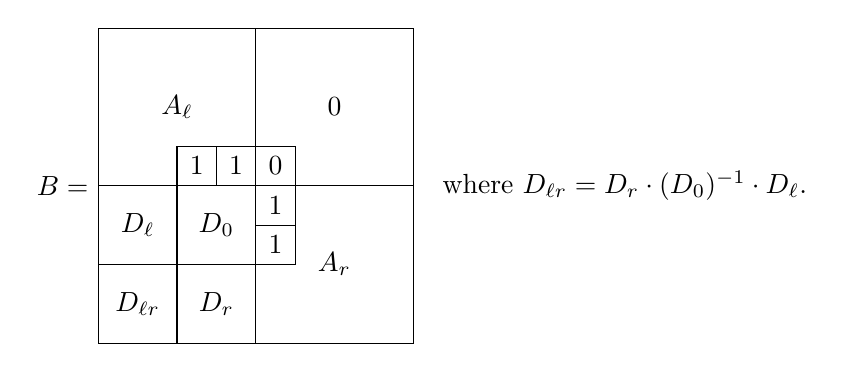
\begin{tikzpicture}
            \begin{scope}[scale=0.5, shift={(0, -4)}]
                \node[anchor=east] at (0, 4) {$B =$};
                \draw (0, 0) -- (8, 0) -- (8, 8) -- (0, 8) -- cycle;
                \draw (0, 4) -- (8, 4);
                \draw (4, 0) -- (4, 8);
                \draw (0, 2) -- (5, 2) -- (5, 5) -- (2, 5) -- (2, 0);
                \draw (3, 4) -- (3, 5);
                \draw (4, 3) -- (5, 3);
                \node at (2, 6) {$A_{\ell}$};
                \node at (6, 2) {$A_{r}$};
                \node at (6, 6) {$0$};
                \node at (1, 1) {$D_{\ell r}$};
                \node at (1, 3) {$D_{\ell}$};
                \node at (3, 1) {$D_{r}$};
                \node at (3, 3) {$D_{0}$};
                \node at (2.5, 4.5) {$1$};
                \node at (3.5, 4.5) {$1$};
                \node at (4.5, 4.5) {$0$};
                \node at (4.5, 3.5) {$1$};
                \node at (4.5, 2.5) {$1$};
            \end{scope}
            \node[anchor=west] at (4.25, 0) {where $D_{\ell r} = D_{r} \cdot (D_{0})^{-1} \cdot D_{\ell}$.};
        \end{tikzpicture}
    \end{center}
    Here $x_{2} \in X_{\ell}$, $x_{0}, x_{1} \in X_{r}$, $y_{0}, y_{1} \in Y_{\ell}$, $y_{2} \in Y_{r}$, $A_{\ell} \in \mathbb{Z}_{2}^{X_{\ell} \times Y_{\ell}}$, $A_{r} \in \mathbb{Z}_{2}^{X_{r} \times Y_{r}}$, $D_{\ell} \in \mathbb{Z}_{2}^{\{x_{0}, x_{1}\} \times (Y_{\ell} \setminus \{y_{0}, y_{1}\})}$, $D_{r} \in \mathbb{Z}_{2}^{(X_{r} \setminus \{x_{0}, x_{1}\}) \times \{y_{0}, y_{1}\}}$, $D_{\ell r} \in \mathbb{Z}_{2}^{(X_{r} \setminus \{x_{0}, x_{1}\}) \times (Y_{\ell} \setminus \{y_{0}, y_{1}\})}$, $D_{0} \in \mathbb{Z}_{2}^{\{x_{0}, x_{1}\} \times \{y_{0}, y_{1}\}}$. The indexing is consistent everywhere.

    Note that $D_{0}$ is non-singular by construction, so $D_{\ell r}$ and $B$ are well-defined. Moreover, a non-singular $\mathbb{Z}_{2}^{2 \times 2}$ matrix is either  $\begin{bmatrix} 1 & 0 \\ 0 & 1 \end{bmatrix}$ or $\begin{bmatrix} 1 & 1 \\ 0 & 1 \end{bmatrix}$ up to re-indexing. Thus, Definition~\ref{def:three_sum_matrix} can be equivalently restated with $D_{0}$ required to be non-singular and $B_{\ell}$, $B_{r}$, and $B$ re-indexed appropriately.
\end{definition}

\begin{definition}
    \label{def:three_sum_matroid}
    \uses{def:three_sum_matrix,StandardRepr}
    % \lean{}
    \leanok
    A matroid $M$ is a $3$-sum of matroids $M_{\ell}$ and $M_{r}$ if there exist standard $\mathbb{Z}_{2}$ representation matrices $B$, $B_{\ell}$, and $B_{r}$ (for $M$, $M_{\ell}$, and $M_{r}$, respectively) of the form given in Definition~\ref{def:three_sum_matrix}.
\end{definition}


\section{Canonical Signing}

\begin{definition}
    \label{def:three_sum_signing_S}
    % \uses{}
    % \lean{}
    \leanok
    We call $D_{0}' \in \mathbb{Q}^{\{x_{0}, x_{1}\} \times \{y_{0}, y_{1}\}}$ the canonical signing of $D_{0} \in \mathbb{Z}_{2}^{\{x_{0}, x_{1}\} \times \{y_{0}, y_{1}\}}$ if
    \[
        D_{0} = \begin{bmatrix}
            1 & 0 \\
            0 & 1 \\
        \end{bmatrix}
        \quad \text{and} \quad
        D_{0}' = \begin{bmatrix}
            1 & 0 \\
            0 & -1
        \end{bmatrix},
        \quad \text{or} \quad
        D_{0} = \begin{bmatrix}
            1 & 1 \\
            0 & 1
        \end{bmatrix}
        \quad \text{and} \quad
        D_{0}' = \begin{bmatrix}
            1 & 1 \\
            0 & 1
        \end{bmatrix}.
    \]
    Similarly, we call $S' \in \mathbb{Q}^{\{x_{0}, x_{1}, x_{2}\} \times \{y_{0}, y_{1}, y_{2}\}}$ the canonical signing of $S \in \mathbb{Z}_{2}^{\{x_{0}, x_{1}, x_{2}\} \times \{y_{0}, y_{1}, y_{2}\}}$ if
    \begin{center}
        \noindent
        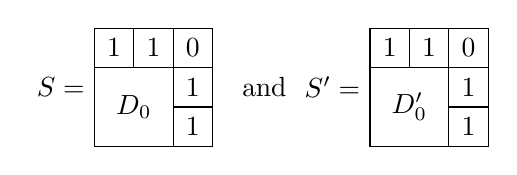
\begin{tikzpicture}
            \begin{scope}[scale=0.5, shift={(-3.5, -1.5)}]
                \node[anchor=east] at (0, 1.5) {$S =$};
                \draw (0, 0) -- (3, 0) -- (3, 3) -- (0, 3) -- cycle;
                \draw (0, 2) -- (3, 2);
                \draw (2, 0) -- (2, 3);
                \draw (1, 2) -- (1, 3);
                \draw (2, 1) -- (3, 1);
                \node at (1, 1) {$D_{0}$};
                \node at (0.5, 2.5) {$1$};
                \node at (1.5, 2.5) {$1$};
                \node at (2.5, 2.5) {$0$};
                \node at (2.5, 1.5) {$1$};
                \node at (2.5, 0.5) {$1$};
            \end{scope}
            \node[anchor=west] at (0, 0) {and};
            \begin{scope}[scale=0.5, shift={(3.5, -1.5)}]
                \node[anchor=east] at (0, 1.5) {$S' =$};
                \draw (0, 0) -- (3, 0) -- (3, 3) -- (0, 3) -- cycle;
                \draw (0, 2) -- (3, 2);
                \draw (2, 0) -- (2, 3);
                \draw (1, 2) -- (1, 3);
                \draw (2, 1) -- (3, 1);
                \node at (1, 1) {$D_{0}'$};
                \node at (0.5, 2.5) {$1$};
                \node at (1.5, 2.5) {$1$};
                \node at (2.5, 2.5) {$0$};
                \node at (2.5, 1.5) {$1$};
                \node at (2.5, 0.5) {$1$};
            \end{scope}
        \end{tikzpicture}
    \end{center}
    To simplify notation, going forward we use $D_{0}$, $D_{0}'$, $S$, and $S'$ to refer to the matrices of the form above.
\end{definition}

\begin{lemma}
    \label{lem:three_sum_signing_S_TU}
    \uses{def:three_sum_signing_S,Matrix.IsTotallyUnimodular}
    % \lean{}
    \leanok
    The canonical signing $S'$ of $S$ (from Definition~\ref{def:three_sum_signing_S}) is TU.
\end{lemma}

\begin{proof}
    % \uses{}
    % \leanok
    Verified via a direct calculation.
\end{proof}

\begin{lemma}
    \label{lem:three_sum_re_signing_helper}
    \uses{Matrix.IsTuSigningOf,def:three_sum_signing_S}
    % \lean{}
    \leanok
    Let $Q$ be a TU signing of $S$ (from Definition~\ref{def:three_sum_signing_S}). Let $u \in \{0, \pm 1\}^{\{x_{0}, x_{1}, x_{2}\}}$, $v \in \{0, \pm 1\}^{\{y_{0}, y_{1}, y_{2}\}}$, and $Q'$ be defined as follows:
    \begin{align*}
        u(i) &= \begin{cases}
            Q (x_{2}, y_{0}) \cdot Q (x_{0}, y_{0}), & i = x_{0}, \\
            Q (x_{2}, y_{0}) \cdot Q (x_{0}, y_{0}) \cdot Q (x_{0}, y_{2}) \cdot Q (x_{1}, y_{2}), & i = x_{1}, \\
            1, & i = x_{2}, \\
        \end{cases} \\
        v(j) &= \begin{cases}
            Q (x_{2}, y_{0}), & j = y_{0}, \\
            Q (x_{2}, y_{1}), & j = y_{1}, \\
            Q (x_{2}, y_{0}) \cdot Q (x_{0}, y_{0}) \cdot Q (x_{0}, y_{2}), & j = y_{2}, \\
        \end{cases} \\
        Q' (i, j) &= Q (i, j) \cdot u(i) \cdot v(j) \quad \forall i \in \{x_{0}, x_{1}, x_{2}\}, \ \forall j \in \{y_{0}, y_{1}, y_{2}\}.
    \end{align*}
    Then $Q' = S'$ (from Definition~\ref{def:three_sum_signing_S}).
\end{lemma}

\begin{proof}
    \uses{Matrix.IsTuSigningOf,Matrix.IsTotallyUnimodular.mul_rows,Matrix.IsTotallyUnimodular.mul_cols,Matrix.IsTotallyUnimodular}
    % \leanok
    Since $Q$ is a TU signing of $S$ and $Q'$ is obtained from $Q$ by multiplying rows and columns by $\pm 1$ factors, $Q'$ is also a TU signing of $S$. By construction, we have
    \begin{align*}
        Q' (x_{2}, y_{0}) &= Q (x_{2}, y_{0}) \cdot 1 \cdot Q (x_{2}, y_{0}) = 1, \\
        Q' (x_{2}, y_{1}) &= Q (x_{2}, y_{1}) \cdot 1 \cdot Q (x_{2}, y_{1}) = 1, \\
        Q' (x_{2}, y_{2}) &= 0, \\
        Q' (x_{0}, y_{0}) &= Q (x_{0}, y_{0}) \cdot (Q (x_{2}, y_{0}) \cdot Q (x_{0}, y_{0})) \cdot Q (x_{2}, y_{0}) = 1, \\
        Q' (x_{0}, y_{1}) &= Q (x_{0}, y_{1}) \cdot (Q (x_{2}, y_{0}) \cdot Q (x_{0}, y_{0})) \cdot Q (x_{2}, y_{1}), \\
        Q' (x_{0}, y_{2}) &= Q (x_{0}, y_{2}) \cdot (Q (x_{2}, y_{0}) \cdot Q (x_{0}, y_{0})) \cdot (Q (x_{2}, y_{0}) \cdot Q (x_{0}, y_{0}) \cdot Q (x_{0}, y_{2})) = 1, \\
        Q' (x_{1}, y_{0}) &= 0, \\
        Q' (x_{1}, y_{1}) &= Q (x_{1}, y_{1}) \cdot (Q (x_{2}, y_{0}) \cdot Q (x_{0}, y_{0}) \cdot Q (x_{0}, y_{2}) \cdot Q (x_{1}, y_{2})) \cdot (Q (x_{2}, y_{1})), \\
        Q' (x_{1}, y_{2}) &= Q (x_{1}, y_{2}) \cdot (Q (x_{2}, y_{0}) \cdot Q (x_{0}, y_{0}) \cdot Q (x_{0}, y_{2}) \cdot Q (x_{1}, y_{2})) \cdot (Q (x_{2}, y_{0}) \cdot Q (x_{0}, y_{0}) \cdot Q (x_{0}, y_{2})) = 1.
    \end{align*}
    Thus, it remains to show that $Q' (x_{0}, y_{1}) = S' (x_{0}, y_{1})$ and $Q' (x_{1}, y_{1}) = S' (x_{1}, y_{1})$.

    Consider the entry $Q' (x_{0}, y_{1})$. If $D_{0} (x_{0}, y_{1}) = 0$, then $Q' (x_{0}, y_{1}) = 0 = S' (x_{0}, y_{1})$. Otherwise, we have $D_{0} (x_{0}, y_{1}) = 1$, and so $Q' (x_{0}, y_{1}) \in \{\pm 1\}$, as $Q'$ is a signing of $S$. If $Q' (x_{0}, y_{1}) = -1$, then
    \[
        \det Q' (\{x_{0}, x_{2}\}, \{y_{0}, y_{1}\}) = \det \begin{bmatrix} 1 & -1 \\ 1 & 1 \end{bmatrix} = 2 \notin \{0, \pm 1\},
    \]
    which contradicts TUness of $Q'$. Thus, $Q' (x_{0}, y_{1}) = 1 = S' (x_{0}, y_{1})$.

    Consider the entry $Q' (x_{1}, y_{1})$. Since $Q'$ is a signing of $S$, we have $Q' (x_{1}, y_{1}) \in \{\pm 1\}$. Consider two cases.
    \begin{enumerate}
        \item Suppose that $D_{0} = \begin{bmatrix} 1 & 0 \\ 0 & 1 \end{bmatrix}$. If $Q' (x_{1}, y_{1}) = 1$, then
        $
            \det Q = \det \begin{bmatrix}
                1 & 1 & 0 \\
                1 & 0 & 1 \\
                0 & 1 & 1
            \end{bmatrix} = -2 \notin \{0, \pm 1\},
        $
        which contradicts TUness of $Q'$. Thus, $Q' (x_{1}, y_{1}) = -1 = S' (x_{1}, y_{1})$.
        \item Suppose that $D_{0} = \begin{bmatrix} 1 & 1 \\ 0 & 1 \end{bmatrix}$. If $Q' (x_{1}, y_{1}) = -1$, then
        $
            \det Q (\{x_{0}, x_{1}\}, \{y_{1}, y_{2}\}) = \det \begin{bmatrix}
                1 & 1 \\
                -1 & 1
            \end{bmatrix} = 2 \notin \{0, \pm 1\},
        $
        which contradicts TUness of $Q'$. Thus, $Q' (x_{1}, y_{1}) = 1 = S' (x_{1}, y_{1})$.
    \end{enumerate}
\end{proof}

\begin{definition}
    \label{def:three_sum_re_signing}
    \uses{Matrix.IsTotallyUnimodular}
    % \lean{}
    \leanok
    Let $X$ and $Y$ be sets with $\{x_{0}, x_{1}, x_{2}\} \subseteq X$ and $\{y_{0}, y_{1}, y_{2}\} \subseteq Y$. Let $Q \in \mathbb{Q}^{X \times Y}$ be a TU matrix. Define $u \in \{0, \pm 1\}^{X}$, $v \in \{0, \pm 1\}^{Y}$, and $Q'$ as follows:
    \begin{align*}
        u(i) &= \begin{cases}
            Q (x_{2}, y_{0}) \cdot Q (x_{0}, y_{0}), & i = x_{0}, \\
            Q (x_{2}, y_{0}) \cdot Q (x_{0}, y_{0}) \cdot Q (x_{0}, y_{2}) \cdot Q (x_{1}, y_{2}), & i = x_{1}, \\
            1, & i = x_{2}, \\
            1, & i \in X \setminus \{x_{0}, x_{1}, x_{2}\},
        \end{cases} \\
        v(j) &= \begin{cases}
            Q (x_{2}, y_{0}), & j = y_{0}, \\
            Q (x_{2}, y_{1}), & j = y_{1}, \\
            Q (x_{2}, y_{0}) \cdot Q (x_{0}, y_{0}) \cdot Q (x_{0}, y_{2}), & j = y_{2}, \\
            1, & j \in Y \setminus \{y_{0}, y_{1}, y_{2}\}, \\
        \end{cases} \\
        Q' (i, j) &= Q (i, j) \cdot u(i) \cdot v(j) \quad \forall i \in X, \ \forall j \in Y.
    \end{align*}
    We call $Q'$ the canonical re-signing of $Q$.
\end{definition}

\begin{lemma}
    \label{lem:three_sum_re_signing_apply}
    \uses{Matrix.IsTuSigningOf,def:three_sum_signing_S,def:three_sum_re_signing}
    % \lean{}
    \leanok
    Let $X$ and $Y$ be sets with $\{x_{0}, x_{1}, x_{2}\} \subseteq X$ and $\{y_{0}, y_{1}, y_{2}\} \subseteq Y$. Let $Q \in \mathbb{Q}^{X \times Y}$ be a TU signing of $Q_{0} \in \mathbb{Z}_{2}^{X \times Y}$ such that $Q_{0} (\{x_{0}, x_{1}, x_{2}\}, \{y_{0}, y_{1}, y_{2}\}) = S$ (from Definition~\ref{def:three_sum_signing_S}). Then the canonical re-signing $Q'$ of $Q$ (from Definition~\ref{def:three_sum_re_signing}) is a TU signing of $Q_{0}$ and $Q' (\{x_{0}, x_{1}, x_{2}\}, \{y_{0}, y_{1}, y_{2}\}) = S'$ (from Definition~\ref{def:three_sum_signing_S}).
\end{lemma}

\begin{proof}
    \uses{Matrix.IsTuSigningOf,Matrix.IsTotallyUnimodular.mul_rows,Matrix.IsTotallyUnimodular.mul_cols,lem:three_sum_re_signing_helper}
    % \leanok
    Since $Q$ is a TU signing of $Q_{0}$ and $Q'$ is obtained from $Q$ by multiplying some rows and columns by $\pm 1$ factors, $Q'$ is also a TU signing of $Q_{0}$. Equality $Q' (\{x_{0}, x_{1}, x_{2}\}, \{y_{0}, y_{1}, y_{2}\}) = S'$ follows from Lemma~\ref{lem:three_sum_re_signing_helper}.
\end{proof}

\begin{definition}
    \label{def:three_sum_signing_B}
    \uses{def:three_sum_matrix,Matrix.IsTuSigningOf,def:three_sum_re_signing}
    % \lean{}
    \leanok
    Suppose that $B_{\ell}$ and $B_{r}$ from Definition~\ref{def:three_sum_matrix} have TU signings $B_{\ell}'$ and $B_{r}'$, respectively. Let $B_{\ell}''$ and $B_{r}''$ be the canonical re-signings (from Definition~\ref{def:three_sum_re_signing}) of $B_{\ell}'$ and $B_{r}'$, respectively. Let $A_{\ell}''$, $A_{r}''$, $D_{\ell}''$, $D_{r}''$, and $D_{0}''$ be blocks of $B_{\ell}''$ and $B_{r}''$ analogous to blocks $A_{\ell}$, $A_{r}$, $D_{\ell}$, $D_{r}$, and $D_{0}$ of $B_{\ell}$ and $B_{r}$. The canonical signing $B''$ of $B$ is defined as
    \begin{center}
        \noindent
        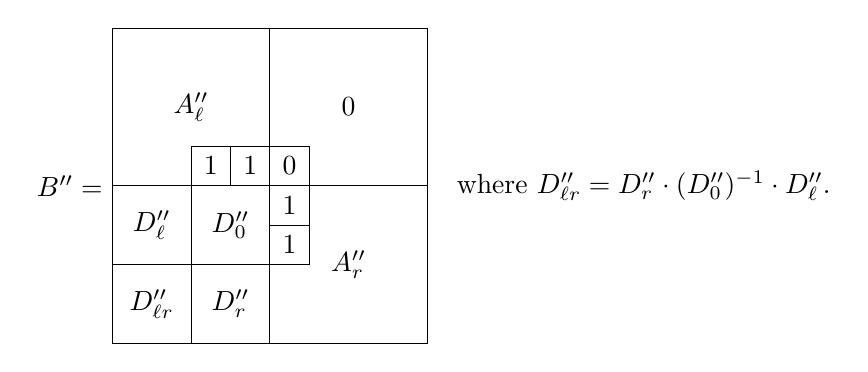
\begin{tikzpicture}
            \begin{scope}[scale=0.5, shift={(0, -4)}]
                \node[anchor=east] at (0, 4) {$B'' =$};
                \draw (0, 0) -- (8, 0) -- (8, 8) -- (0, 8) -- cycle;
                \draw (0, 4) -- (8, 4);
                \draw (4, 0) -- (4, 8);
                \draw (0, 2) -- (5, 2) -- (5, 5) -- (2, 5) -- (2, 0);
                \draw (3, 4) -- (3, 5);
                \draw (4, 3) -- (5, 3);
                \node at (2, 6) {$A_{\ell}''$};
                \node at (6, 2) {$A_{r}''$};
                \node at (6, 6) {$0$};
                \node at (1, 1) {$D_{\ell r}''$};
                \node at (1, 3) {$D_{\ell}''$};
                \node at (3, 1) {$D_{r}''$};
                \node at (3, 3) {$D_{0}''$};
                \node at (2.5, 4.5) {$1$};
                \node at (3.5, 4.5) {$1$};
                \node at (4.5, 4.5) {$0$};
                \node at (4.5, 3.5) {$1$};
                \node at (4.5, 2.5) {$1$};
            \end{scope}
            \node[anchor=west] at (4.25, 0) {where $D_{\ell r}'' = D_{r}'' \cdot (D_{0}'')^{-1} \cdot D_{\ell}''$.};
        \end{tikzpicture}
    \end{center}
    Note that $D_{0}''$ is non-singular by construction, so $D_{\ell r}''$ and hence $B''$ are well-defined.
\end{definition}


\section{Properties of Canonical Signing}

\begin{lemma}
    \label{lem:three_sum_signing_B_valid}
    \uses{def:three_sum_signing_B}
    % \lean{}
    \leanok
    $B''$ from Definition~\ref{def:three_sum_signing_B} is a signing of $B$.
\end{lemma}

\begin{proof}
    \uses{lem:three_sum_re_signing_apply,Matrix.IsTuSigningOf}
    % \leanok
    By Lemma~\ref{lem:three_sum_re_signing_apply}, $B_{\ell}''$ and $B_{r}''$ are TU signings of $B_{\ell}$ and $B_{r}$, respectively. As a result, blocks $A_{\ell}''$, $A_{r}''$, $D_{\ell}''$, $D_{r}''$, and $D_{0}''$ in $B''$ are signings of the corresponding blocks in $B$. Thus, it remains to show that $D_{\ell r}''$ is a signing of $D_{\ell r}$. This can be verified via a direct calculation. \todo{Need details?}
\end{proof}

\begin{lemma}
    \label{lem:three_sum_signing_B_r_props}
    \uses{def:three_sum_matrix,Matrix.IsTuSigningOf,def:three_sum_re_signing}
    % \lean{}
    \leanok
    Suppose that $B_{r}$ from Definition~\ref{def:three_sum_matrix} has a TU signing $B_{r}'$. Let $B_{r}''$ be the canonical re-signing (from Definition~\ref{def:three_sum_re_signing}) of $B_{r}'$. Let $c_{0}'' = B_{r}'' (X_{r}, y_{0})$, $c_{1}'' = B_{r}'' (X_{r}, y_{1})$, and $c_{2}'' = c_{0}'' - c_{1}''$. Then the following statements hold.
    \begin{enumerate}
        \item\label{item:tss_Brp_c01} For every $i \in X_{r}$, $\begin{bmatrix} c_{0}'' (i) & c_{1}'' (i) \end{bmatrix} \in \{0, \pm 1\}^{\{y_{0}, y_{1}\}} \setminus \left\{ \begin{bmatrix} 1 & -1 \end{bmatrix}, \begin{bmatrix} -1 & 1 \end{bmatrix} \right\}$.
        \item\label{item:tss_Brp_c2} For every $i \in X_{r}$, $c_{2}'' (i) \in \{0, \pm 1\}$.
        \item\label{item:tss_Brp_tu1} $\begin{bmatrix} c_{0}'' & c_{2}'' & A_{r}'' \end{bmatrix}$ is TU.
        \item\label{item:tss_Brp_tu2} $\begin{bmatrix} c_{1}'' & c_{2}'' & A_{r}'' \end{bmatrix}$ is TU.
        \item\label{item:tss_Brp_tu3} $\begin{bmatrix} c_{0}'' & c_{1}'' & c_{2}'' & A_{r}'' \end{bmatrix}$ is TU.
    \end{enumerate}
\end{lemma}

\begin{proof}
    \uses{lem:three_sum_re_signing_apply,Matrix.IsTotallyUnimodular,Matrix.shortTableauPivot,Matrix.IsTotallyUnimodular.shortTableauPivot,Matrix.IsTotallyUnimodular.mul_rows,Matrix.IsTotallyUnimodular.mul_cols}
    % \leanok
    Throughout the proof we use that $B_{r}''$ is TU, which holds by Lemma~\ref{lem:three_sum_re_signing_apply}.

    \begin{enumerate}
        \item Since $B_{r}''$ is TU, all its entries are in $\{0, \pm 1\}$, and in particular $\begin{bmatrix} c_{0}'' (i) & c_{1}'' (i) \end{bmatrix} \in \{0, \pm 1\}^{\{y_{0}, y_{1}\}}$. If $\begin{bmatrix} c_{0}' (i) & c_{1}'' (i) \end{bmatrix} = \begin{bmatrix} 1 & -1 \end{bmatrix}$, then
        \[
            \det B_{r}'' (\{x_{2}, i\}, \{y_{0}, y_{1}\}) = \det \begin{bmatrix} 1 & 1 \\ 1 & -1 \end{bmatrix} = -2 \notin \{0, \pm 1\},
        \]
        which contradicts TUness of $B_{r}''$. Similarly, if $\begin{bmatrix} c_{0}'' (i) & c_{1}'' (i) \end{bmatrix} = \begin{bmatrix} -1 & 1 \end{bmatrix} $, then
        \[
            \det B_{r}'' (\{x_{2}, i\}, \{y_{0}, y_{1}\}) = \det \begin{bmatrix} 1 & 1 \\ -1 & 1 \end{bmatrix} = 2 \notin \{0, \pm 1\},
        \]
        which contradicts TUness of $B_{r}''$. Thus, the desired statement holds.

        \item Follows from item~\ref{item:tss_Brp_c01} and a direct calculation.

        \item Performing a short tableau pivot in $B_{r}''$ on $(x_{2}, y_{0})$ yields:
        \[
            B_{r}'' = \begin{bmatrix}
                \fbox{1} & 1 & 0 \\
                c_{0} & c_{1} & A_{r}
            \end{bmatrix}
            \quad \to \quad
            \begin{bmatrix}
                1 & 1 & 0 \\
                -c_{0} & c_{1}'' - c_{0} & A_{r}
            \end{bmatrix}
        \]
        The resulting matrix can be transformed into $\begin{bmatrix} c_{0}'' & c_{2}'' & A_{r}'' \end{bmatrix}$ by removing row $x_{2}$ and multiplying columns $y_{0}$ and $y_{1}$ by $-1$. Since $B_{r}''$ is TU and since TUness is preserved under pivoting, taking submatrices, multiplying columns by ${\pm 1}$ factors, we conclude that $\begin{bmatrix} c_{0}'' & c_{2}'' & A_{r}'' \end{bmatrix}$ is TU.

        \item Similar to item~\ref{item:tss_Brp_tu2}, performing a short tableau pivot in $B_{r}''$ on $(x_{2}, y_{1})$ yields:
        \[
            B_{r}'' = \begin{bmatrix}
                1 & \fbox{1} & 0 \\
                c_{0} & c_{1} & A_{r}
            \end{bmatrix}
            \quad \to \quad
            \begin{bmatrix}
                1 & 1 & 0 \\
                c_{0}'' - c_{1} & -c_{1} & A_{r}
            \end{bmatrix}
        \]
        The resulting matrix can be transformed into $\begin{bmatrix} c_{1}'' & c_{2}'' & A_{r}'' \end{bmatrix}$ by removing row $x_{2}$, multiplying column $y_{1}$ by $-1$, and swapping the order of columns $y_{0}$ and $y_{1}$. Since $B_{r}''$ is TU and since TUness is preserved under pivoting, taking submatrices, multiplying columns by ${\pm 1}$ factors, and re-ordering columns, we conclude that $\begin{bmatrix} c_{1}'' & c_{2}'' & A_{r}'' \end{bmatrix}$ is TU.

        \item Let $V$ be a square submatrix of $\begin{bmatrix} c_{0}'' & c_{1}'' & c_{2}'' & A_{r}'' \end{bmatrix}$. Our goal is to show that $\det V \in \{0, \pm 1\}$.

        Suppose that column $c_{2}''$ is not in $V$. Then $V$ is a submatrix of $B_{r}''$, which is TU. Thus, $\det V \in \{0, \pm 1\}$. Going forward we assume that column $z$ is in $V$.

        Suppose that columns $c_{0}''$ and $c_{1}''$ are both in $V$. Then $V$ contains columns $c_{0}''$, $c_{1}''$, and $c_{2}'' = c_{0}'' - c_{1}''$, which are linearly. Thus, $\det V = 0$. Going forward we assume that at least one of the columns $c_{0}''$ and $c_{1}''$ is not in $V$.

        Suppose that column $c_{1}''$ is not in $V$. Then $V$ is a submatrix of $\begin{bmatrix} c_{0}'' & c_{2}'' & A_{r}'' \end{bmatrix}$, which is TU by item~\ref{item:tss_Brp_tu1}. Thus, $\det V \in \{0, \pm 1\}$. Similarly, if column $c_{0}''$ is not in $V$, then $V$ is a submatrix of $\begin{bmatrix} c_{1}'' & c_{2}'' & A_{r}'' \end{bmatrix}$, which is TU by item~\ref{item:tss_Brp_tu2}. Thus, $\det V \in \{0, \pm 1\}$.

    \end{enumerate}
\end{proof}

\begin{lemma}
    \label{lem:three_sum_signing_B_l_props}
    \uses{def:three_sum_matrix,Matrix.IsTuSigningOf,def:three_sum_re_signing}
    % \lean{}
    \leanok
    Suppose that $B_{\ell}$ from Definition~\ref{def:three_sum_matrix} has a TU signing $B_{\ell}'$. Let $B_{\ell}''$ be the canonical re-signing (from Definition~\ref{def:three_sum_re_signing}) of $B_{\ell}'$. Let $d_{0}'' = B_{\ell}'' (x_{0}, Y_{\ell})$, $d_{1}'' = B_{\ell}'' (x_{1}, Y_{\ell})$, and $d_{2}'' = d_{0}'' - d_{1}''$. Then the following statements hold.
    \begin{enumerate}
        \item\label{item:tss_Blp_d01} For every $j \in Y_{\ell}$, $\begin{bmatrix} d_{0}'' (i) \\ d_{1}'' (j) \end{bmatrix} \in \{0, \pm 1\}^{\{x_{0}, x_{1}\}} \setminus \left\{ \begin{bmatrix} 1 \\ -1 \end{bmatrix}, \begin{bmatrix} -1 \\ 1 \end{bmatrix} \right\}$.
        \item\label{item:tss_Blp_d2} For every $j \in Y_{\ell}$, $d_{2}'' (j) \in \{0, \pm 1\}$.
        \item\label{item:tss_Blp_tu1} $\begin{bmatrix} A_{\ell}'' \\ d_{0}'' \\ d_{2}'' \end{bmatrix}$ is TU.
        \item\label{item:tss_Blp_tu2} $\begin{bmatrix} A_{\ell}'' \\ d_{1}'' \\ d_{2}'' \end{bmatrix}$ is TU.
        \item\label{item:tss_Blp_tu3} $\begin{bmatrix} A_{\ell}'' \\ d_{0}'' \\ d_{1}'' \\ d_{2}'' \end{bmatrix}$ is TU.
    \end{enumerate}
\end{lemma}

\begin{proof}
    \uses{lem:three_sum_signing_B_r_props}
    % \leanok
    Apply Lemma~\ref{lem:three_sum_signing_B_r_props} to $B_{\ell}^{\top}$, or repeat the same arguments up to transposition.
\end{proof}

\begin{lemma}
    \label{lem:three_sum_signing_B_props}
    \uses{def:three_sum_signing_B,Matrix.IsTotallyUnimodular}
    % \lean{}
    \leanok
    Let $B''$ be from Definition~\ref{def:three_sum_signing_B}. Let $c_{0}'' = B'' (X_{r}, y_{0})$, $c_{1}'' = B'' (X_{r}, y_{1})$, and $c_{2}'' = c_{0}'' - c_{1}''$. Similarly, let $d_{0}'' = B'' (x_{0}, Y_{\ell})$, $d_{1}'' = B'' (x_{1}, Y_{\ell})$, and $d_{2}'' = d_{0}'' - d_{1}''$. Then the following statements hold.
    \begin{enumerate}
        \item\label{item:tss_Bp_c2} For every $i \in X_{r}$, $c_{2}'' (i) \in \{0, \pm 1\}$.
        \item\label{item:tss_Bp_Deq} If $D_{0}'' = \begin{bmatrix} 1 & 0 \\ 0 & -1 \end{bmatrix}$, then $D'' = c_{0}'' \otimes d_{0}'' - c_{1}'' \otimes d_{1}''$. If $D_{0}'' = \begin{bmatrix} 1 & 1 \\ 0 & 1 \end{bmatrix}$, then $D'' = c_{0}'' \otimes d_{0}'' - c_{0}'' \otimes d_{1}'' + c_{1}'' \otimes d_{1}''$.
        \item\label{item:tss_Bp_Dcols} For every $j \in Y_{\ell}$, $D'' (X_{r}, j) \in \{0, \pm c_{0}'', \pm c_{1}'', \pm c_{2}''\}$.
        \item\label{item:tss_Bp_Drows} For every $i \in X_{r}$, $D'' (i, Y_{\ell}) \in \{0, \pm d_{0}'', \pm d_{1}'', \pm d_{2}''\}$.
        \item\label{item:tss_Bp_DAr} $\begin{bmatrix} D'' & A_{r}'' \end{bmatrix}$ is TU.
        \item\label{item:tss_Bp_AlD} $\begin{bmatrix} A_{\ell}'' \\ D'' \end{bmatrix}$ is TU.
    \end{enumerate}
\end{lemma}

\begin{proof}
    \uses{lem:three_sum_signing_B_r_props,lem:three_sum_signing_B_l_props,Matrix.IsTotallyUnimodular}
    % \leanok
    \begin{enumerate}
        \item Holds by Lemma~\ref{lem:three_sum_signing_B_r_props}.\ref{item:tss_Brp_c2}.

        \item Note that
        \[
            \begin{bmatrix} D_{\ell}'' \\ D_{\ell r}'' \end{bmatrix} = \begin{bmatrix} D_{0}'' \\ D_{r}'' \end{bmatrix} \cdot (D_{0}'')^{-1} \cdot D_{\ell}'', \quad
            \begin{bmatrix} D_{0}'' \\ D_{r}'' \end{bmatrix} = \begin{bmatrix} D_{0}'' \\ D_{r}'' \end{bmatrix} \cdot (D_{0}'')^{-1} \cdot D_{0}'', \quad
            \begin{bmatrix} D_{0}'' \\ D_{r}'' \end{bmatrix} = \begin{bmatrix} c_{0}'' & c_{1}'' \end{bmatrix}, \quad
            \begin{bmatrix} D_{\ell}'' & D_{0}'' \end{bmatrix} = \begin{bmatrix} d_{0}'' \\ d_{1}'' \end{bmatrix}.
        \]
        Thus,
        \[
            D''
            = \begin{bmatrix} D_{\ell}'' & D_{0}'' \\ D_{\ell r}'' & D_{r}'' \end{bmatrix}
            = \begin{bmatrix} D_{0}'' \\ D_{r}'' \end{bmatrix} \cdot (D_{0}'')^{-1} \cdot \begin{bmatrix} D_{\ell}'' & D_{0}'' \end{bmatrix}
            = \begin{bmatrix} c_{0}'' & c_{1}'' \end{bmatrix} \cdot (D_{0}'')^{-1} \cdot \begin{bmatrix} d_{0}'' \\ d_{1}'' \end{bmatrix}.
        \]
        Considering the two cases for $D_{0}''$ and performing the calculations yields the desired results.
        % If $D_{0}'' = \begin{bmatrix} 1 & 0 \\ 0 & -1 \end{bmatrix}$, then $(D_{0}'')^{-1} = \begin{bmatrix} 1 & 0 \\ 0 & -1 \end{bmatrix}$, and the formula above yields $D'' = c_{0}'' \otimes d_{0}'' - c_{1}'' \otimes d_{1}''$. If $D_{0}'' = \begin{bmatrix} 1 & 1 \\ 0 & 1 \end{bmatrix}$, then $(D_{0}'')^{-1} = \begin{bmatrix} 1 & -1 \\ 0 & 1 \end{bmatrix}$, and the formula above yields $D'' = c_{0}'' \otimes d_{0}'' - c_{0}'' \otimes d_{1}'' + c_{1}'' \otimes d_{1}''$.

        \item Let $j \in Y_{\ell}$. By Lemma~\ref{lem:three_sum_signing_B_l_props}.\ref{item:tss_Blp_d01}, $\begin{bmatrix} d_{0}'' (i) \\ d_{1}'' (j) \end{bmatrix} \in \{0, \pm 1\}^{\{x_{0}, x_{1}\}} \setminus \left\{ \begin{bmatrix} 1 \\ -1 \end{bmatrix}, \begin{bmatrix} -1 \\ 1 \end{bmatrix} \right\}$. Consider two cases.
        \begin{enumerate}
            \item If $D_{0}'' = \begin{bmatrix} 1 & 0 \\ 0 & -1 \end{bmatrix}$, then by item~\ref{item:tss_Bp_Deq} we have $D'' (X_{r}, j) = d_{0}'' (j) \cdot c_{0}''  + (-d_{1}'' (j)) \cdot c_{1}''$. By considering all possible cases for $d_{0}'' (j)$ and $d_{1}'' (j)$, we conclude that $D'' (X_{r}, j) \in \{0, \pm c_{0}'', \pm c_{1}'', \pm (c_{0}'' - c_{1}'')\}$.
            \item If $D_{0}'' = \begin{bmatrix} 1 & 1 \\ 0 & 1 \end{bmatrix}$, then by item~\ref{item:tss_Bp_Deq} we have $D'' (X_{r}, j) = (d_{0}'' (j) - d_{1}'' (j)) \cdot c_{0}''  + d_{1}'' (j) \cdot c_{1}''$. By considering all possible cases for $d_{0}'' (j)$ and $d_{1}'' (j)$, we conclude that $D'' (X_{r}, j) \in \{0, \pm c_{0}'', \pm c_{1}'', \pm (c_{0}'' - c_{1}'')\}$.
        \end{enumerate}

        \item Let $i \in X_{r}$. By Lemma~\ref{lem:three_sum_signing_B_r_props}.\ref{item:tss_Brp_c01}, $\begin{bmatrix} c_{0}'' (i) & c_{1}'' (i) \end{bmatrix} \in \{0, \pm 1\}^{\{y_{0}, y_{1}\}} \setminus \left\{ \begin{bmatrix} 1 & -1 \end{bmatrix}, \begin{bmatrix} -1 & 1 \end{bmatrix} \right\}$. Consider two cases.
        \begin{enumerate}
            \item If $D_{0}'' = \begin{bmatrix} 1 & 0 \\ 0 & -1 \end{bmatrix}$, then by item~\ref{item:tss_Bp_Deq} we have $D'' (i, Y_{\ell}) = c_{0}'' (i) \cdot d_{0}''  + (-c_{1}'' (i)) \cdot d_{1}''$. By considering all possible cases for $c_{0}'' (i)$ and $c_{1}'' (i)$, we conclude that $D'' (i, Y_{\ell}) \in \{0, \pm d_{0}'', \pm d_{1}'', \pm d_{2}''\}$.
            \item If $D_{0}'' = \begin{bmatrix} 1 & 1 \\ 0 & 1 \end{bmatrix}$, then by item~\ref{item:tss_Bp_Deq} we have $D'' (i, Y_{\ell}) = c_{0}'' (i) \cdot d_{0}'' + (c_{1}'' (i) - c_{0}'' (i)) \cdot d_{1}''$. By considering all possible cases for $c_{0}'' (i)$ and $c_{1}'' (i)$, we conclude that $D'' (i, Y_{\ell}) \in \{0, \pm d_{0}'', \pm d_{1}'', \pm d_{2}''\}$.
        \end{enumerate}

        \item By Lemma~\ref{lem:three_sum_signing_B_r_props}.\ref{item:tss_Brp_tu3}, $\begin{bmatrix} c_{0}'' & c_{1}'' & c_{2}'' & A_{r}'' \end{bmatrix}$ is TU. Since TUness is preserved under adjoining zero columns, copies of existing columns, and multiplying columns by $\pm 1$ factors, $\begin{bmatrix} 0 & \pm c_{0}'' & \pm c_{1}'' & \pm c_{2}'' & A_{r}'' \end{bmatrix}$ is also TU. By item~\ref{item:tss_Bp_Dcols}, $\begin{bmatrix} D'' & A_{r}'' \end{bmatrix}$ is a submatrix of the latter matrix, hence it is also TU.

        \item By Lemma~\ref{lem:three_sum_signing_B_l_props}.\ref{item:tss_Blp_tu3}, $\begin{bmatrix} A_{\ell}'' \\ d_{0}'' \\ d_{1}'' \\ d_{2}'' \end{bmatrix}$ is TU. Since TUness is preserved under adjoining zero rows, copies of existing rows, and multiplying rows by $\pm 1$ factors, $\begin{bmatrix} A_{\ell}'' \\ 0 \\ \pm d_{0}'' \\ \pm d_{1}'' \\ \pm d_{2}'' \end{bmatrix}$ is also TU. By item~\ref{item:tss_Bp_Drows}, $\begin{bmatrix} A_{\ell}'' \\ D'' \end{bmatrix}$ is a submatrix of the latter matrix, hence it is also TU.
    \end{enumerate}
\end{proof}


\section{Proof of Regularity}

\begin{definition}
    \label{def:three_sum_like_matrix}
    \uses{Matrix.IsTotallyUnimodular}
    % \lean{}
    \leanok
    Let $X_{\ell}$, $Y_{\ell}$, $X_{r}$, $Y_{r}$ be sets and let $c_{0}, c_{1} \in \mathbb{Q}^{X_{r}}$ be column vectors such that for every $i \in X_{r}$ we have $c_{0} (i), \ c_{1} (i), \ c_{0} (i) - c_{1} (i) \in \{0, \pm 1\}$. Define $\mathcal{C} (X_{\ell}, Y_{\ell}, X_{r}, Y_{r}; c_{0}, c_{1})$ to be the family of matrices of the form $\begin{bmatrix} A_{\ell} & 0 \\ D & A_{r} \end{bmatrix}$ where $A_{\ell} \in \mathbb{Q}^{X_{\ell} \times Y_{\ell}}$, $A_{r} \in \mathbb{Q}^{X_{r} \times Y_{r}}$, and $D \in \mathbb{Q}^{X_{r} \times Y_{\ell}}$ are such that:
    \begin{enumerate}
        \item\label{item:tsl_cols} for every $j \in Y_{\ell}$, $D (X_{r}, j) \in \{0, \pm c_{0}, \pm c_{1}, \pm (c_{0} - c_{1})\}$,
        \item\label{item:tsl_bot} $\begin{bmatrix} c_{0} & c_{1} & c_{0} - c_{1} & A_{r} \end{bmatrix}$ is TU,
        \item\label{item:tsl_left} $\begin{bmatrix} A_{\ell} \\ D \end{bmatrix}$ is TU.
    \end{enumerate}
\end{definition}

\begin{lemma}
    \label{lem:three_sum_like_signing_B}
    \uses{def:three_sum_signing_B,def:three_sum_like_matrix}
    % \lean{}
    \leanok
    Let $B''$ be from Definition~\ref{def:three_sum_signing_B}. Then $B'' \in \mathcal{C} (X_{\ell}, Y_{\ell}, X_{r}, Y_{r}; c_{0}'', c_{1}'')$ where $c_{0}'' = B'' (X_{r}, y_{0})$ and $c_{1}'' = B'' (X_{r}, y_{1})$.
\end{lemma}

\begin{proof}
    \uses{lem:three_sum_signing_B_props,def:three_sum_like_matrix}
    % \leanok
    Recall that $c_{0}'' - c_{1}'' \in \{0, \pm 1\}^{X_{r}}$ by Lemma~\ref{lem:three_sum_signing_B_props}.\ref{item:tss_Bp_c2}, so $\mathcal{C} (X_{\ell}, Y_{\ell}, X_{r}, Y_{r}; c_{0}'', c_{1}'')$ is well-defined. To see that $B'' \in \mathcal{C} (X_{\ell}, Y_{\ell}, X_{r}, Y_{r}; c_{0}'', c_{1}'')$, note that all properties from Definition~\ref{def:three_sum_like_matrix} are satisfied: property~\ref{item:tsl_cols} holds by Lemma~\ref{lem:three_sum_signing_B_props}.\ref{item:tss_Bp_Dcols}, property~\ref{item:tsl_bot} holds by Lemma~\ref{lem:three_sum_signing_B_r_props}.\ref{item:tss_Brp_tu3}, and property~\ref{item:tsl_left} holds by Lemma~\ref{lem:three_sum_signing_B_props}.\ref{item:tss_Bp_AlD}.
\end{proof}

\begin{lemma}
    \label{lem:three_sum_like_pivot}
    \uses{def:three_sum_like_matrix,Matrix.shortTableauPivot}
    % \lean{}
    \leanok
    Let $C \in \mathcal{C} (X_{\ell}, Y_{\ell}, X_{r}, Y_{r}; c_{0}, c_{1})$ from Definition~\ref{def:three_sum_like_matrix}. Let $x \in X_{\ell}$ and $y \in Y_{\ell}$ be such that $A_{\ell} (x, y) \neq 0$, and let $C'$ be the result of performing a short tableau pivot in $C$ on $(x, y)$. Then $C' \in \mathcal{C} (X_{\ell}, Y_{\ell}, X_{r}, Y_{r}; c_{0}, c_{1})$.
\end{lemma}

\begin{proof}
    \uses{Matrix.shortTableauPivot_zero,Matrix.IsTotallyUnimodular,Matrix.IsTotallyUnimodular.shortTableauPivot}
    % \leanok
    Our goal is to show that $C'$ satisfies all properties from Definition~\ref{def:three_sum_like_matrix}. Let $C' = \begin{bmatrix} C_{11}' & C_{12}' \\ C_{21}' & C_{22}' \end{bmatrix}$, and let $\begin{bmatrix} A_{\ell}' \\ D' \end{bmatrix}$ be the result of performing a short tableau pivot on $(x, y)$ in $\begin{bmatrix} A_{\ell} \\ D \end{bmatrix}$. Observe the following.

    \begin{itemize}
        \item By Lemma~\ref{Matrix.shortTableauPivot_zero}, $C_{11}' = A_{\ell}'$, $C_{12}' = 0$, $C_{21}' = D'$, and $C_{22}' = A_{r}$.
        \item Since $\begin{bmatrix} A_{\ell} \\ D \end{bmatrix}$ is TU by property~\ref{item:tsl_left} for $C$, all entries of $A_{\ell}$ are in $\{0, \pm 1\}$.
        \item $A_{\ell} (x, y) \in \{\pm 1\}$, as $A_{\ell} (x, y) \in \{0, \pm 1\}$ by the above observation and $A_{\ell} (x, y) \neq 0$ by the assumption.
        \item Since $\begin{bmatrix} A_{\ell} \\ D \end{bmatrix}$ is TU by property~\ref{item:tsl_left} for $C$, and since pivoting preserves TUness, $\begin{bmatrix} A_{\ell}' \\ D' \end{bmatrix}$ is also TU.
    \end{itemize}

    These observations immediately imply properties~\ref{item:tsl_bot} and~\ref{item:tsl_left} for $C'$. Indeed, property~\ref{item:tsl_bot} holds for $C'$, since $C_{22}' = A_{r}$ and $\begin{bmatrix} c_{0} & c_{1} & c_{0} - c_{1} & A_{r} \end{bmatrix}$ is TU by property~\ref{item:tsl_bot} for $C$. On the other hand, property~\ref{item:tsl_left} follows from $C_{11}' = A_{\ell}'$, $C_{21}' = D'$, and $\begin{bmatrix} A_{\ell}' \\ D' \end{bmatrix}$ being TU. Thus, it only remains to show that $C'$ satisfies property~\ref{item:tsl_cols}. Let $j \in Y_{r}$. Our goal is to prove that $D' (X_{r}, j) \in \{0, \pm c_{0}, \pm c_{1}, \pm (c_{0} - c_{1})\}$.

    Suppose $j = y$. By the pivot formula, $D' (X_{r}, y) = -\frac{D (X_{r}, y)}{A_{\ell} (x, y)}$. Since $D (X_{r}, y) \in \{0, \pm c_{0}, \pm c_{1}, \pm (c_{0} - c_{1})\}$ by property~\ref{item:tsl_cols} for $C$ and since $A_{\ell} (x, y) \in \{\pm 1\}$, we get $D' (X_{r}, y) \in \{0, \pm c_{0}, \pm c_{1}, \pm (c_{0} - c_{1})\}$.

    Now suppose $j \in Y_{\ell} \setminus \{y\}$. By the pivot formula, $D' (X_{r}, j) = D (X_{r}, j) - \frac{A_{\ell} (x, j)}{A_{\ell} (x, y)} \cdot D (X_{r}, y)$. Here $D (X_{r}, j), \ D (X_{r}, y) \in \{0, \pm c_{0}, \pm c_{1}, \pm (c_{0} - c_{1})\}$ by property~\ref{item:tsl_cols} for $C$, and $A_{\ell} (x, j) \in \{0, \pm 1\}$ and $A_{\ell} (x, y) \in \{\pm 1\}$ by the prior observations. Perform an exhaustive case distinction on $D (X_{r}, j)$, $D (X_{r}, y)$, $A_{\ell} (x, j)$, and $A_{\ell} (x, y)$. In every case, we can show that either $\begin{bmatrix} A_{\ell} (x, y) & A_{\ell} (x, j) \\ D (X_{r}, y) & D (X_{r}, j) \end{bmatrix}$ contains a submatrix with determinant not in $\{0, \pm 1\}$, which contradicts TUness of $\begin{bmatrix} A_{\ell} \\ D \end{bmatrix}$, or that $D' (X_{r}, j) \in \{0, \pm c_{0}, \pm c_{1}, \pm (c_{0} - c_{1})\}$, as desired. \todo{need details?}
\end{proof}

\begin{lemma}
    \label{lem:three_sum_like_tu}
    \uses{def:three_sum_like_matrix,Matrix.IsTotallyUnimodular}
    % \lean{}
    \leanok
    Let $C \in \mathcal{C} (X_{\ell}, Y_{\ell}, X_{r}, Y_{r}; c_{0}, c_{1})$ from Definition~\ref{def:three_sum_like_matrix}. Then $C$ is TU.
\end{lemma}

\begin{proof}
    \uses{def:three_sum_like_matrix,Matrix.isTotallyUnimodular_iff_forall_isPartiallyUnimodular,shortTableauPivot_submatrix_det_ni_signTypeCastRange,lem:three_sum_like_pivot}
    % \leanok
    By Lemma~\ref{Matrix.isTotallyUnimodular_iff_forall_isPartiallyUnimodular}, it suffices to show that $C$ is $k$-PU for every $k \in \mathbb{N}$. We prove this claim by induction on $k$. The base case with $k = 1$ holds, since properties~\ref{item:tsl_bot} and~\ref{item:tsl_left} in Definition~\ref{def:three_sum_like_matrix} imply that $A_{\ell}$, $A_{r}$, and $D$ are TU, so all their entries of $C = \begin{bmatrix} A_{\ell} & 0 \\ D & A_{r} \end{bmatrix}$ are in $\{0, \pm 1\}$, as desired.

    Suppose that for some $k \in \mathbb{N}$ we know that every $C' \in \mathcal{C} (X_{\ell}, Y_{\ell}, X_{r}, Y_{r}; c_{0}, c_{1})$ is $k$-PU. Our goal is to show that $C$ is $(k + 1)$-PU, i.e., that every $(k + 1) \times (k + 1)$ submatrix $S$ of $C$ has $\det V \in \{0, \pm 1\}$.

    First, suppose that $V$ has no rows in $X_{\ell}$. Then $V$ is a submatrix of $\begin{bmatrix} D & A_{r} \end{bmatrix}$, which is TU by property~\ref{item:tsl_bot} in Definition~\ref{def:three_sum_like_matrix}, so $\det V \in \{0, \pm 1\}$. Thus, we may assume that $S$ contains a row $x_{\ell} \in X_{\ell}$.

    Next, note that without loss of generality we may assume that there exists $y_{\ell} \in Y_{\ell}$ such that $V (x_{\ell}, y_{\ell}) \neq 0$. Indeed, if $V (x_{\ell}, y) = 0$ for all $y$, then $\det V = 0$ and we are done, and $V (x_{\ell}, y) = 0$ holds whenever $y \in Y_{r}$.

    Since $C$ is $1$-PU, all entries of $V$ are in $\{0, \pm 1\}$, and hence $V (x_{\ell}, y_{\ell}) \in \{\pm 1\}$. Thus, by Lemma~\ref{shortTableauPivot_submatrix_det_ni_signTypeCastRange}, performing a short tableau pivot in $V$ on $(x_{\ell}, y_{\ell})$ yields a matrix that contains a $k \times k$ submatrix $S''$ such that $|\det V| = |\det V''|$. Since $V$ is a submatrix of $C$, matrix $V''$ is a submatrix of the matrix $C'$ resulting from performing a short tableau pivot in $C$ on the same entry $(x_{\ell}, y_{\ell})$. By Lemma~\ref{lem:three_sum_like_pivot}, we have $C' \in \mathcal{C} (X_{\ell}, Y_{\ell}, X_{r}, Y_{r}; c_{0}, c_{1})$. Thus, by the inductive hypothesis applied to $V''$ and $C'$, we have $\det V'' \in \{0, \pm 1\}$. Since $|\det V| = |\det V''|$, we conclude that $\det V \in \{0, \pm 1\}$.
\end{proof}

\begin{lemma}
    \label{lem:three_sum_signing_B_tu}
    \uses{def:three_sum_signing_B,Matrix.IsTotallyUnimodular}
    % \lean{}
    \leanok
    $B''$ from Definition~\ref{def:three_sum_signing_B} is TU.
\end{lemma}

\begin{proof}
    \uses{lem:three_sum_like_signing_B,lem:three_sum_like_tu}
    % \leanok
    Combine the results of Lemmas~\ref{lem:three_sum_like_signing_B} and~\ref{lem:three_sum_like_tu}.
    % By Lemma~\ref{lem:three_sum_like_signing_B}, $B'' \in \mathcal{C} (X_{\ell}, Y_{\ell}, X_{r}, Y_{r}; c_{0}'', c_{1}'')$, and by Lemma~\ref{lem:three_sum_like_tu}, every matrix in $\mathcal{C} (X_{\ell}, Y_{\ell}, X_{r}, Y_{r}; c_{0}'', c_{1}'')$ is TU.
\end{proof}

\begin{theorem}
    \label{thm:matroid_three_sum_regular}
    \uses{def:three_sum_matroid,Matroid.IsRegular}
    % \lean{}
    \leanok
    Let $M$ be a $3$-sum of regular matroids $M_{\ell}$ and $M_{r}$. Then $M$ is also regular.
\end{theorem}

\begin{proof}
    \uses{StandardRepr,def:three_sum_matroid,StandardRepr.toMatroid_isRegular_iff_hasTuSigning,def:three_sum_signing_B,lem:three_sum_signing_B_valid,lem:three_sum_signing_B_tu}
    % \leanok
    Let $B$, $B_{\ell}$, and $B_{r}$ be standard $\mathbb{Z}_{2}$ representation matrices from Definition~\ref{def:three_sum_matroid}. Since $M_{\ell}$ and $M_{r}$ are regular, by Lemma~\ref{StandardRepr.toMatroid_isRegular_iff_hasTuSigning}, $B_{\ell}$ and $B_{r}$ have TU signings. Then the canonical signing $B''$ from Definition~\ref{def:three_sum_signing_B} is a TU signing of $B$. Indeed, $B''$ is a signing of $B$ by Lemma~\ref{lem:three_sum_signing_B_valid}, and $B''$ is TU by Lemma~\ref{lem:three_sum_signing_B_tu}. Thus, $M$ is regular by Lemma~\ref{StandardRepr.toMatroid_isRegular_iff_hasTuSigning}.
\end{proof}
